\documentclass[12pt]{book}

\usepackage[utf8]{inputenc}
\usepackage{amsthm,amsmath,amssymb}
\usepackage{graphicx}
\usepackage{enumitem}
%\usepackage{pifont}
\usepackage{dirtytalk}
%\usepackage{hhline}
\usepackage{xcolor}
\usepackage{hyperref}
%\usepackage{dsfont}
\usepackage{tcolorbox}
\usepackage{xfrac}
\usepackage{units}
%\usepackage{cancel}
%\usepackage{float}
%\usepackage{isotope}







\usepackage{caption}
\captionsetup{labelfont=bf, font={small,sf}, margin=\parindent, labelsep=period}
\captionsetup[figure]{name=Fig.\kern-0.6ex}
\captionsetup[table]{name=Tab.\kern-0.6ex}


\makeatletter
\newcommand{\lambdabar}{{\mathchoice
  {\smash@bar\textfont\displaystyle{0.25}{1.2}\lambda}
  {\smash@bar\textfont\textstyle{0.25}{1.2}\lambda}
  {\smash@bar\scriptfont\scriptstyle{0.25}{1.2}\lambda}
  {\smash@bar\scriptscriptfont\scriptscriptstyle{0.25}{1.2}\lambda}
}}
\newcommand{\smash@bar}[4]{%
  \smash{\rlap{\raisebox{-#3\fontdimen5#10}{$\m@th#2\mkern#4mu\mathchar'26$}}}%
}
\makeatother


\theoremstyle{definition}
\newtheorem*{defi}{\bfseries Definition}
\newtheorem*{theo}{\bfseries Theorem}
\newtheorem*{expl}{\bfseries Example}
\newtheorem*{prf}{Proof:}



\setcounter{tocdepth}{2}


\hypersetup{colorlinks=true, linkcolor=blue, filecolor=magenta, urlcolor=cyan}


% \usepackage[style=numeric]{biblatex}
% \addbibresource{lecturenotes.bib}




\newcommand{\R}{\mathbb R}
\newcommand{\Z}{\mathbb Z}
\newcommand{\Q}{\mathbb Q}
\newcommand{\C}{\mathbb C}
\newcommand{\N}{\mathbb N}
\renewcommand{\v}[1]{\vec{#1}}
\newcommand{\e}{\varepsilon}
\newcommand{\de}{\delta}
\newcommand{\p}{\varphi}
\newcommand{\norm}[1]{\left\Vert {#1}\right\Vert}
\newcommand{\scalar}[1]{\left\langle {#1}\right\rangle}
\newcommand{\bM}{\begin{pmatrix}}
\newcommand{\eM}{\end{pmatrix}}
\newcommand{\abs}[1]{\left\vert {#1}\right\vert}
\let\oldsum\sum
\renewcommand{\sum}[2]{\oldsum\limits_{#1}^{#2}}
\let\shortto\to
\renewcommand{\to}{\longrightarrow}
\let\mapsto\shortmapsto
\newcommand{\mapsto}{\longmapsto}
\newcommand{\si}{\sigma}
\newcommand{\del}[2][]{\dfrac{\partial {#1}}{\partial {#2}}}
\newcommand{\der}[2][]{\dfrac{d {#1}}{d {#2}}}
\newcommand{\para}[1]{\left( {#1} \right)}
\newcommand{\bra}[1]{\langle {#1} \vert}
\newcommand{\ket}[1]{\vert {#1} \rangle}
\renewcommand{\qed}{\hfill\ding{112}}


\let\d\dontneetu
\DeclareMathOperator{\tr}{tr}
\DeclareMathOperator{\d}{d}
\let\Re\mathfrakR
\let\Im\mathfrakI
\DeclareMathOperator{\Re}{Re}
\DeclareMathOperator{\Im}{Im}
\DeclareMathOperator{\mat}{Mat}



\begin{document}
\begin{titlepage}

\newcommand{\HRule}{\rule{\linewidth}{0.5mm}}
\center

\textsc{\LARGE Uppsala University}\\[1.5cm]
% 
\includegraphics[scale=.5]{fig/Uppsala_University_seal_svg.png}\\[1cm]
\textsc{\Large Quantum Information}\\[0.5cm]
\textsc{\large }\\[0.5cm]


\HRule \\[0.4cm]
{\huge \bfseries Lecture Notes}\\[0.4cm]
\HRule \\[1.5cm]

\begin{minipage}{0.4\textwidth}
\begin{flushleft} \large
\emph{Author:}\\
Louis \textsc{Henkel}\\
\end{flushleft}

\end{minipage}\\[2cm]


{\large \today}\\[2cm]
\vfill

\end{titlepage}
\tableofcontents


\chapter{Introduction}
\section*{Quantum Theory}

One can say, that quantum theory is a probability theory where events are assotiated with complex numbers $\alpha$ called probability amplitudes. There are three rules for these probability amplitudes:
\begin{enumerate}[label = (\alph*)]
  \item Born rule: $P = \abs{\alpha}^2$ gives the probability of the event $\alpha$
  \item For a sequence of events with amplitude $\alpha_1, \cdots, \alpha_n$, then the amplitude of the whole sequence is: $\prod\limits_{i=1}^{n} \alpha_{N-i+1}$
  \item For two interconnected events with amplitude $\alpha_1$ and $\alpha_2$, then the probability of one event occuring if the other has occured, then the amplitude of this event is $\alpha = \alpha_1 + \alpha_2$. The probability of such event is given by:
  \begin{equation}
    P = \abs{\alpha_1}^2 + \abs{\alpha_2}^2 + 2 \Re(\alpha_1^*\alpha_2)
  \end{equation}
  where the mixed term is called the interference term. This is where the difference between classical information and quantum information theory lies.
\end{enumerate}

\section*{Qubits}
A qubit is a quantum mechanical system that can be described as a two dimensional Hilbert space. In general, this can be the polarisation of a photon, spin of an electron, of a neutron and so on. We can view a qubit as a abstract sense as $\mathcal H = \mathrm{span}\{\ket{0}, \ket{1}\}$. An arbitrary qubit state as $\alpha_0 \ket{0} + \alpha_1 \ket{1}$ with $\alpha_i \in \C$, with the normalisation condition ${\alpha_0}^1 + \abs{\alpha_1}^2 = 1$. From the normalisation we can write the probability amplitudes as
\begin{equation}
  \begin{cases}
    \alpha_0 = \cos \sfrac \theta 2 e^{i\p_0} \\
    \alpha_1 = \sin \sfrac \theta 2 e^{i\p_1}
  \end{cases}
\end{equation}
This allows us to write a general state $\ket\phi$ as:
\#\begin{align*}
 \ket{\phi} & = \cos \sfrac\theta 2 e^{i\p_0} \ket{0} + \sin \sfrac \theta 2 e^{i\p_1} \ket{0} \\
 & = e^{i\p_0} \para{\cos \sfrac \theta 2 \ket{0} + \sin \sfrac \theta 2 e^{i(\p_1 - \p_0)} \ket{0}} \\
 & \sim \cos \sfrac \theta 2 \ket{0} + \sin \sfrac \theta 2 e^{i\p} \ket{1}
\end{align*}
This can be represented in a sphere called the Bloch sphere
\begin{figure}[h!]
	\centering
  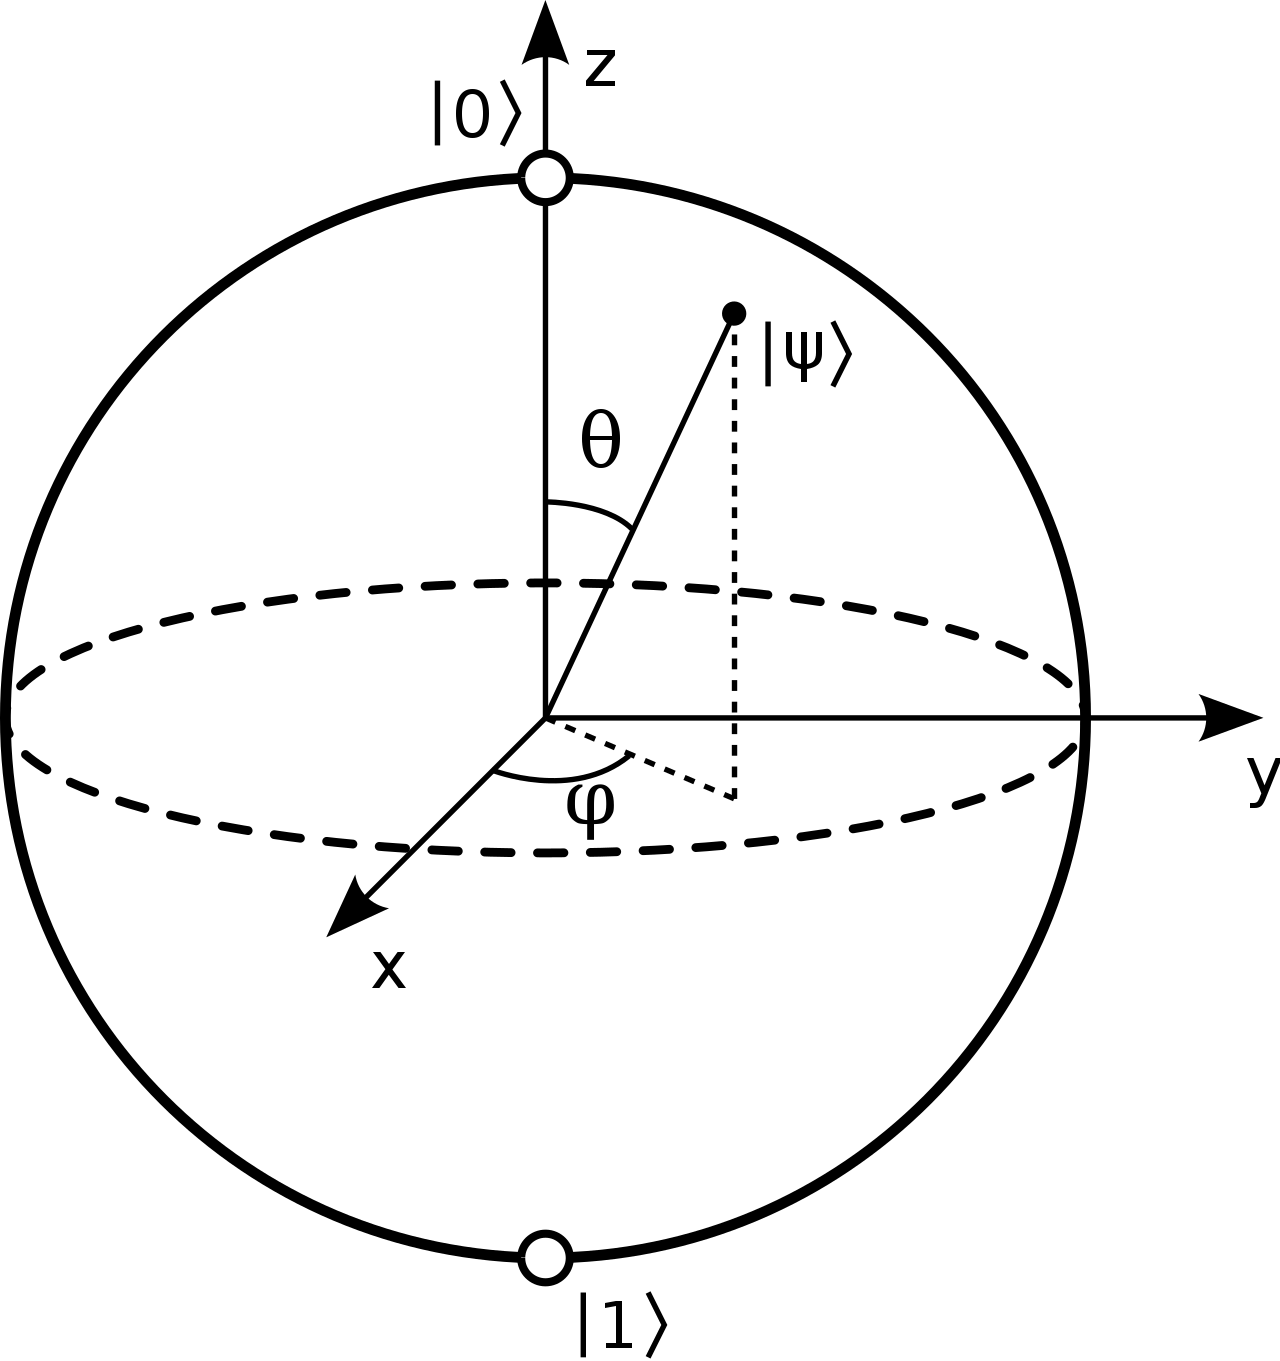
\includegraphics[width=0.4\textwidth]{fig/Bloch_sphere.svg}
  \caption{Representation of a Bloch sphere }%\cite{fig:Bloch-sphere}}
\end{figure}
%% Exkurs about the Hilbert fiber space for global phase factor and bloch sphere in higher dimensions

\chapter{Quantum Mechanics}

\section{Density operator}
Suppose we have a preparation of quantum states (such as sending photons through a polariser), that are not perfect with some impurity. Say that each possible \emph{pure} state $\ket{\Psi_1}, \cdots \ket{\Psi_K}$ with probabilities $P_1, \cdots P_K$. Suppose we measure an observable $A$ throught the operator $\hat A$ on this set of states, and we want to calculate the expectation value of this observable:
\begin{equation}
  A_{\textrm{av}} = \scalar{\hat A}_{\{P_k, \ket{\Psi_k}\}} = \sum{k=1}{K} P_k \scalar{\Psi_k \vert \hat A \vert \Psi_k} \label{eq:av-expectation-val}
\end{equation}
where this $K \in \N \cup \{\infty\}$ \emph{does not have to} be the same as dimension as the Hilbert space of the system. We can rewrite the equation \ref{eq:av-expectation-val} as:
\begin{align*}
 A_{\textrm{av}} & = \sum{k=1}{K} P_k \scalar{\Psi_k \vert \hat A \vert \Psi_k} \\
 & = \oldsum_k \oldsum_n P_k \scalar{\Psi_k \vert n} \scalar{n \vert \hat A \vert \Psi_k} \\
 & = \oldsum_k \oldsum_n P_k \scalar{n \vert \hat A \vert \Psi_k} \scalar{\Psi_k \vert n} \\
 & = \oldsum_k p_k \tr(\hat A \ket{\Psi_k} \bra{\Psi_k}) \\
 & = \tr\para{\hat A \oldsum_k p_k \ket{\Psi_k} \bra{\Psi_k}} \\
 & = \tr(\hat A \hat \rho)
\end{align*}
We define $\hat \rho := \oldsum_k p_k \ket{\Psi_k} \bra{\Psi_k}$ as the density operator representing the ensemble $\{p_k, \ket{\Psi_k}\}$

\subsection{Properties}
\begin{enumerate}[label = \alph*)]
  \item The density operator is a hermitian semi-definit operator: $\scalar{\hat \rho} \geq 0$. \\
  \emph{Proof:}
  \begin{equation*}
    \scalar{\Psi \vert \hat \rho \vert \Psi} = \oldsum_k p_k \abs{\scalar{\Psi \vert k}}^2 \geq 0 \forall \Psi \in \mathcal H
  \end{equation*}
  \item $\tr \hat \rho = 1$
  \item $\hat{\rho}^2 \leq \hat \rho$ and $\hat \rho^2 = \hat \rho \iff \hat \rho = \ket{\Psi_1}\bra{\Psi_1}$ called a pure state.
\end{enumerate}

\subsection{Example: \textrm{Qubit density operator}}
In diagonal (spectral) form, we can write the density operator as:
\begin{equation*}
  \hat \rho = p_0 \ket{\Psi_0}\bra{\Psi_0} + p_1 \ket{\Psi_1}\bra{\Psi_1}
\end{equation*}
where $\scalar{\Psi_0\vert\Psi_1} = 0$ and we can define the states $\Psi_0, \Psi_1$ as:
\begin{align*}
 \Psi_0 & = \cos\sfrac\theta 2 \ket{0} + \sin \sfrac\theta 2 e^{i\p} \ket{1} \\
 \Psi_1 & = - \sin \sfrac\theta 2 e^{-i\p}\ket{0} + \cos \sfrac\theta 2 \ket{1}
\end{align*}
with $p_0 + p_1 = 1$, so we can write these as: $p_0 = \frac{1 + r}{2}$, $p_1 = \frac{1 - r}{2}$, so we can write the density operator as:
\begin{equation}
  \hat \rho = \frac{1}{2} \para{\hat I + \v r \cdot \v \si}
\end{equation}
where $\v r(\sin\theta \cos\p, \sin\theta \sin\p, \cos\theta)$ is a $3D$-vector and $\si$ are the Pauli operators, and represent a point in the Bloch ball. For $r = 0$, the density operator is the identity operator and we have the maximal mixed state.

\section{Mixing theorem}
It was formulated by Hughstom et al. in PLA (1993)
\begin{tcolorbox}
  Consider $\hat \rho = \sum{k=1}{\dim(\mathcal H)} p_k \ket{e_k}\bra{e_k}$, where $\scalar{e_k \vert e_\ell} = \de_{k, \ell}$ and $\hat \eta = \sum{\ell = 1}{L} q_\ell \ket{\phi_\ell}\bra{\phi_\ell}$.
  Then $\hat \rho = \hat \eta$ iff there exists an unitary matrix $V \in \mat(\dim (\mathcal L) \times \dim(\mathcal L))$ such that
  \begin{equation}
  \sqrt{q_\ell} \ket{\phi_\ell} = \sum{k=1}{\dim \mathcal H} \sqrt{p_k} \ket{e_k} V_{kl} \forall l = 1, \cdots, \dim \mathcal H
  \end{equation}
\end{tcolorbox}



\section{Composite Systems}
In quantum mechanics we use tennsor products to describe states of composite systems. Assume me have systems a, b and c with bases, then the wave function of such a composite system can be written as:
\begin{equation}
  \ket{\Psi_{ABC}} = \oldsum_{k\ell m} a_{k\ell m} \ket{a_k} \otimes \ket{b_\ell} \otimes \ket{c_m}
\end{equation}
where the dimension of the Hilbert space is given by
\begin{equation}
  \dim \mathcal H_{ABC} = \dim \mathcal H_A \cdot \mathcal H_B \cdot \mathcal H_C
\end{equation}
is the number of combinations of basis vectors of the subsystems. As a notation we usually write
\begin{equation}
  \ket{a_k} \otimes \ket{b_\ell} \otimes \ket{c_m} \to \ket{a_k b_\ell c_m}
\end{equation}
As terminology: With $N$ subsystems, we mean a $N$ particle composite system.

Assume we have system of $N$ qubits, then the dimension of the composite system
\begin{equation*}
  \mathcal H_{2D}^{\otimes N} = \bigotimes_{i=1}^{N} \mathcal H_{2D}
\end{equation*}
with dimension
\begin{equation}
  \dim \mathcal H_{2D}^{\otimes N} = 2^N
\end{equation}
we can write the basis as binanry strings $x \in \{0, 1\}^N$ of length $N$ that generate the Hilbert space. A general wave function can then be written as
\begin{equation}
  \ket{\Psi_{N\textrm{-Qubit}}} = \sum{x=1}{2^N} c_x \ket{x}
\end{equation}


\subsection{Bipartite case}
In the bipartite case we set $N=2$ with subsystems A and B, an arbitrary pure state is described by
\begin{equation}
  \ket{\Psi^{AB}} = \sum{k=1}{n_A} \sum{\ell = 1}{n_B} a_{k\ell} \ket{k} \otimes \ket{\ell}
\end{equation}
with $n_i = \dim \mathcal H_i$.

%% USe theorem instead
\begin{theo}
It states, that:
\begin{equation}
  \ket{\Psi^{AB}} = \sum{m=1}{\min\{n_A, n_B\}} \sqrt{d_m} \ket{A_m} \otimes \ket{B_m}
\end{equation}
where $\ket{A_m} \in \mathcal H_A$ and $\scalar{A_m \vert A_{n}} = \de_{mn}$ for A and B and $\oldsum_m d_m = 1$.
% END THEOREM
\end{theo}

For the proof we need singular value decomposition: Assume $a \in \mat(n_A \times n_B)$ matrix. Then we can write this matrix $a$ as
\begin{equation*}
  a = U \cdot d \cdots V
\end{equation*}
where $U \in U(n_A)$, $V \in U(n_B)$ unitary matrices and $d$ a \say{diagonal} $n_A \times n_B$ matrix with the singular values $\sqrt{d_i}$ on the diagonal.
% use Proof environement
\begin{prf}

% \emph{Proof:}
We view $a_{k\ell}$ as a $n_A \times n_B$ matrix. Then using singular value decomposition we get
\begin{equation*}
  a_{k\ell} = \sum{m=1}{\min\{n_A, n_B\}} U_{km} \sqrt{d_m} V{m\ell}
\end{equation*}
For a general bipartite wave function we get
\begin{align*}
  \ket{\Psi^{AB}} & = \sum{k=1}{n_A} \sum{\ell=1}{n_B} \sum{m=1}{\min\{n_A, n_B\}} U_{km} \sqrt{d_m} V{m\ell}\: \ket{k} \otimes \ket{\ell} \\
  & = \oldsum_{m} \sqrt{d_m} \oldsum_k U_{km} \ket{k} \otimes \oldsum_\ell V{m\ell} \ket{l} \\
  & = \sum{m=1}{\min\{n_A, n_B\}} \sqrt{d_m} \ket{A_m} \otimes \ket{B_m}
\end{align*}
It remains to prove, that orthonormality of the basis.
\begin{align*}
  \scalar{A_m \vert A_n} & = \sum{k, k'}{n_A} U_{km}^* U_{k'm} \scalar{k \vert k'} \\
  & = \sum{k=1}{n_A} U^\dagger_{mk} U_{kn} \\
  & = (U^\dagger U)_{m, n} = \de_{m,n}
\end{align*}
\end{prf}
%% END PROOF
There exists no generalisation to $N$ partite system. If it existsed it would take the form: $\Psi^{AB\cdots X} = \oldsum_m \sqrt{d_m} \ket{A_m} \cdots \ket{X_m}$

%% BEgin example

% \emph{Example:}
\begin{expl}
Assume we have a 3-state qubit, we can write:
\begin{align*}
  \Psi^{ABC} & = \ket{000} + a \para{\ket{011} + \ket{101} + \ket{110}} \\
  & = \ket{+++} + \ket{---} = \ket{GHZ}
\end{align*}
where $\ket{\pm} = \ket{0} \pm \ket{1}$.

In comparason a state:
\begin{equation*}
  \ket{\Psi^{ABC}} = \ket{111} + a \para{\cdots}
\end{equation*}
that connot be decomposed into a Schmidt form. A similar state is
\begin{equation*}
  \ket{W} := \frac{1}{\sqrt{3}} \para{\ket{001} + \ket{010} + \ket{100}}
\end{equation*}
that has no Schmidt decomposition.
\end{expl}

\section{Reduced denisty operator, partial trace}

Assume we have a bipartite system with state $\ket{\Psi^{AB}}$. What does it mean to only have accoess to onu of the two subsystems, say A? Vhat does it do operationally. Suppose we measure observable $O_A$ an A, then using Schmidt decomposition
\begin{align*}
  \scalar{\hat O_A}_{\Psi^{AB}} & = \scalar{\Psi^{AB} \vert \hat O_A \otimes \hat I_B \vert \Psi^{AB}} \\
  & = \oldsum_{k\ell} \sqrt{d_k} \sqrt{d_\ell} \scalar{A_k \vert \hat O_A \vert A_\ell} \scalar{B_k \vert \hat I \vert B_\ell} \\
  & = \oldsum_{k} d_k \scalar{A_k \vert \hat O_A \vert A_k} \\
  & = \tr\para{O_A \oldsum_k d_k \ket{A_k} \bra{A_k}} \\
  & = \tr\para{O_A \rho_B}
\end{align*}
where $\rho_A$ is the reduced density operator in spectral form. A reduced density operator can be computed as a partial trace:
\begin{equation}
  \rho_A = \tr_A \ket{\Psi^{AB}} \bra{\Psi^{AB}} = \oldsum_m \scalar{B_m \vert \Psi^{AB}} \scalar{\Psi^{AB} \vert B_m}
\end{equation}


\section{Completely positive maps (quantum channels)}
Within the space of all possible states (Bloch sphere for a single qubit), we can have maps between different quantum states. If we restrict ourselves to only using unitary transformation, that pure states can only stay pure states (called \emph{closed system}) whereas completely positive maps that can transform a system more generally.

\begin{defi}
A completely positive map (CMP) $\rho \to \mathcal E(\rho) \geq 0$ satisfies:
\begin{enumerate}[label = (\alph*)]
  \item $\tr[\mathcal E(\rho)]$ is the probability that $\mathcal E$ happens:
  \begin{subequations}
  \begin{equation}
    \Longrightarrow 0 \leq \tr[\mathcal E(\rho)] \leq 1,
  \end{equation}
  with $\tr[\mathcal E(\rho)] = 1$ if the CPM is a completely positive trance perserving (CPTP) map.
  \item A CMP should be linear, so that: $\mathcal E \para{\oldsum_k p_k \rho_k} = \oldsum_k p_k \mathcal E(\rho_k)$.
  \item Let $A, B$ be positive semi-definit operator, then the following inequality should hold
  \begin{equation}
    \mathcal E(A) \geq 0 \qquad \text{(positivity)}
  \end{equation}
  and, if $B$ is an operator that acts on a langer Hilbert space, then
  \begin{equation}
    \mathcal E \otimes \mathcal I(B) \geq 0
  \end{equation}
  for \emph{any} extension of the system (complete positivity). This conditions guaranties that remote systems cannot influence the physical nature of $\mathcal E$
  \end{subequations}
\end{enumerate}
\end{defi}
\begin{defi}
Transposition:
\begin{equation}
\para{\ket{A} \bra{A^\perp}}^T =  \ket{A^\perp}\bra{A}
\end{equation}
(partial transpostion)
\end{defi}

\begin{expl}
We have the state:
\begin{align*}
  \ket{\Psi^{AB}} & = \frac{1}{\sqrt{2}} \para{\ket{01} - \ket{20}} \quad\to\quad \rho_{AB}^{T_A} = \ket{\Psi^{AB}} \bra{\Psi^AB}^{T_A} \\
  & = \frac{1}{2} \para{\ket{01} - \ket{10}}\para{\bra{01} - \bra{10}}^{T_A} \\
  & = \frac{1}{2} \para{\ket{01}\bra{01} - \ket{01}\bra{10} - \ket{10}\bra{01} + \ket{10}\bra{10}}^{T_A} \\
  & = \frac{1}{2} \para{\ket{0}\bra{0} \otimes \ket{1}\bra{1} - \ket{0}\bra{1} \otimes \ket{1} \bra{0} - \ket{0} \bra{1} \otimes \ket{0} \bra{1} + \ket{1}\bra{1} \otimes\ket{0} \bra{0}} \\
  & =
  \begin{pmatrix}
    0 & 0 & 0 & \sfrac{1}{2} \\
    0 & \sfrac{1}{2} & 0 & \\
    0 & 0 & \sfrac{1}{2} & 0 \\
    \sfrac{1}{2} & 0 & 0 & 0
  \end{pmatrix}
\end{align*}
with eigenvalues $\left\{\frac{1}{2}, \frac{1}{2}, \frac{1}{2}, -\frac{1}{2}\right\}$
\end{expl}




\end{document}
